\part{Diferencias Finitas}

Para mejorar la precisión de los resultados, se implementó un modelo de diferencias finitas aplicado a la matriz de potencial hidráulico. De esta manera, se pueden calcular las líneas de flujo, obteniendo así el caudal de infiltración. El objetivo principal es determinar la efectividad de este método frente a un proceso más simple, como el cálculo manual expuesto en la sección anterior.

\section{Teoría}

\subsection{Ley de Darcy}

La ley de Darcy se expresa como:

\begin{equation}
    q = k \cdot i \cdot A
\end{equation}

Lo cual es análogo a:

\begin{equation}
    v = k \cdot i
\end{equation}

Donde \(i\) es el gradiente hidráulico. Discretizando en el espacio, se obtiene lo siguiente:

\begin{equation}
    i = \frac{dh}{dl} = \frac{dh}{dx}; \frac{dh}{dy}; \frac{dh}{dz}
\end{equation}

Sea lo siguiente:

\begin{figure}[H]
    \centering
    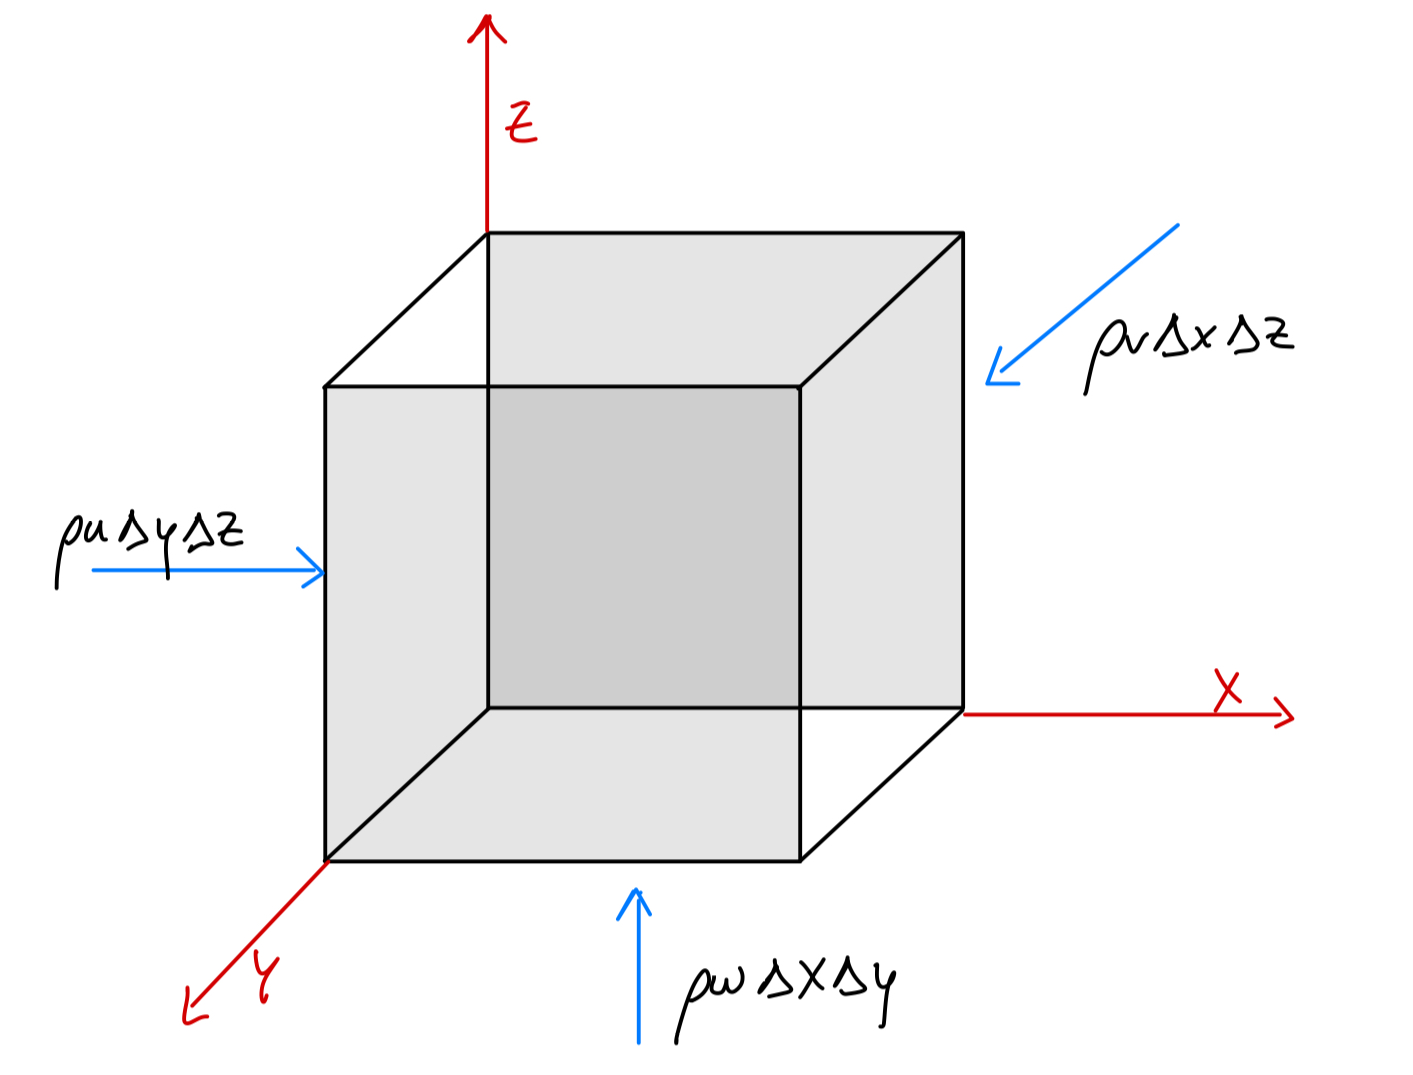
\includegraphics[width=0.5\textwidth]{FOTOS/in.jpg}
    \caption{Entrada al sistema}
    \label{fig:ley_darcy_in}
\end{figure}

La serie de Taylor expone que:

\begin{equation}
    f(x) = f(a) + \frac{df(a) \Delta X}{dx \cdot 1!} + ... + \frac{\Delta X^n}{n!} \cdot \frac{d^n f(a)}{dx^n}
\end{equation}

Por lo tanto, lo que sale del sistema es:

\begin{figure}[H]
    \centering
    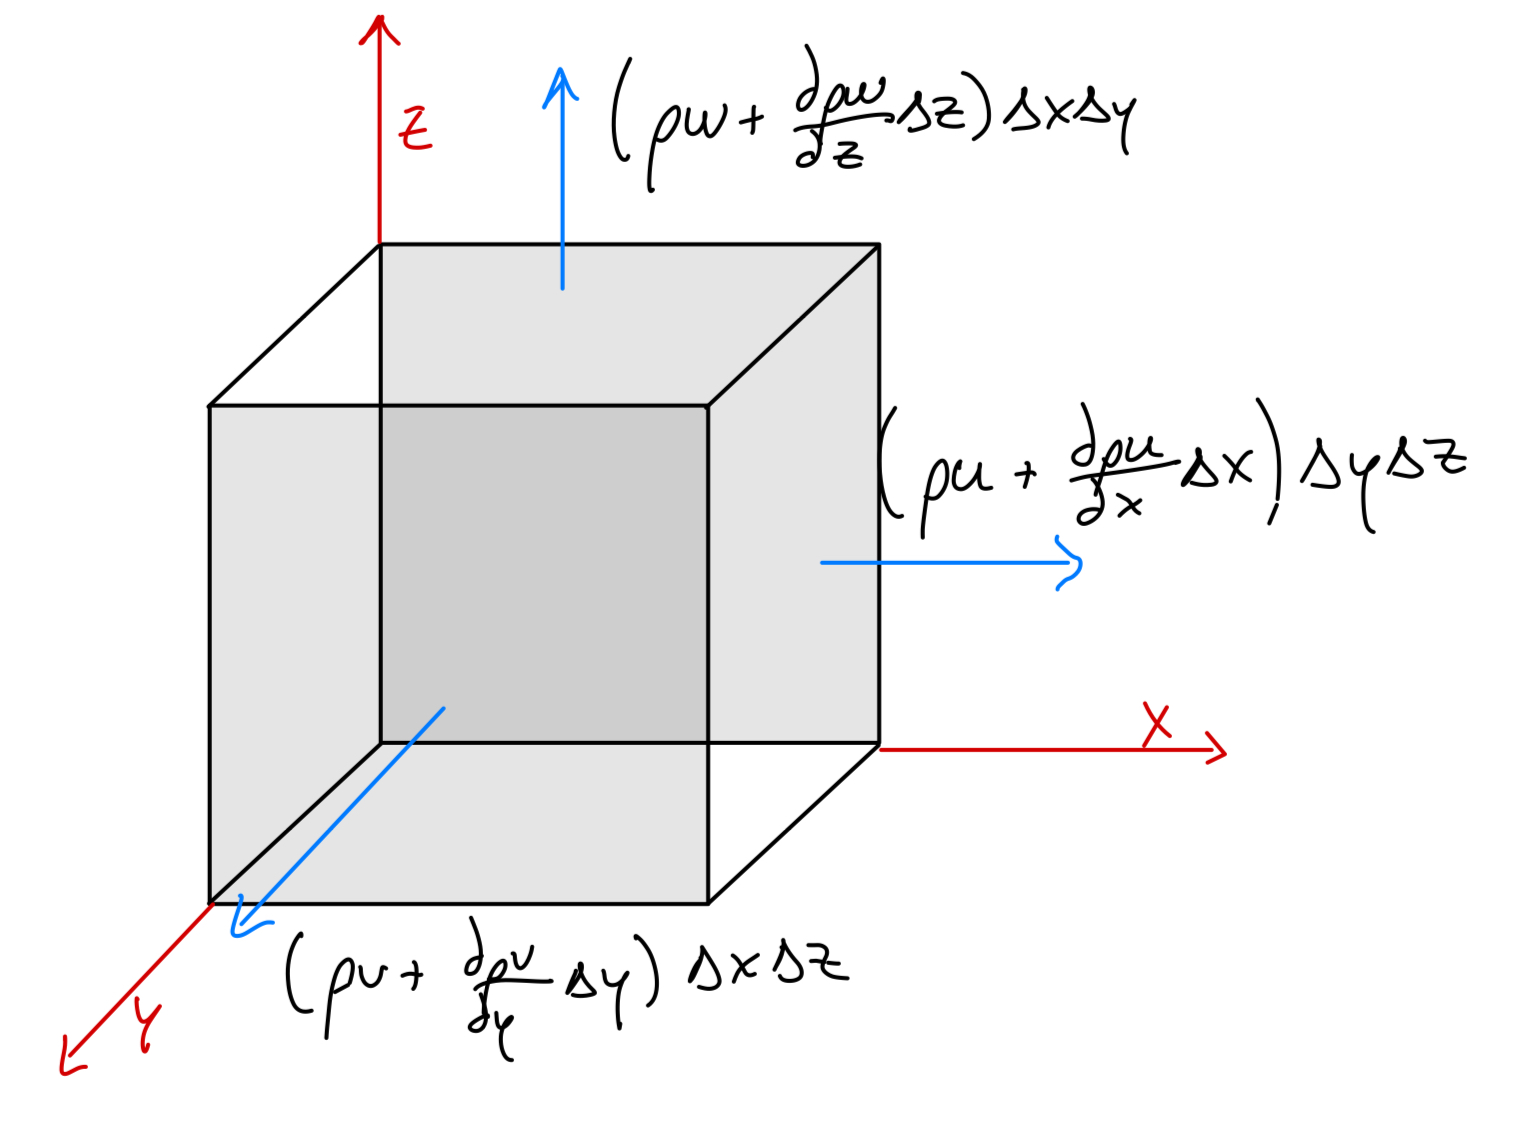
\includegraphics[width=0.5\textwidth]{FOTOS/out.jpg}
    \caption{Salida del sistema}
    \label{fig:ley_darcy_out}
\end{figure}

Luego, por conservación de masa:

\begin{equation}
    Q_{int} = Q_{out}
\end{equation}

De lo que se obtiene:

\begin{equation}
    \rho_u \Delta_y \Delta_z + \rho_v \Delta_x \Delta_z + \rho_w \Delta_x \Delta_y = (\rho_u + \frac{d\rho_u \Delta x}{dx})\Delta_y \Delta_z + (\rho_v + \frac{d\rho_v \Delta y}{dy})\Delta_x \Delta_z + (\rho_w + \frac{d\rho_w \Delta z}{dz})\Delta_x \Delta_y
\end{equation}

Simplificando:

\begin{equation}
    \Delta_x \Delta_y \Delta_z = Volumen
\end{equation}

Dado que el fluido es agua, que es incompresible, se tiene:

\begin{equation}
   -\rho(\frac{du}{dx}+ \frac{dv}{dy}+ \frac{dw}{dz}) = 0
\end{equation}

Lo cual es análogo a:

\begin{equation}
    -\rho \nabla \cdot \vec{v} = 0 = \nabla \cdot \vec{v}
\end{equation}

Por lo tanto, al reemplazar en la ley de Darcy, se obtiene:

\begin{equation}
    V_x = k_x\cdot \frac{dh}{dx}; V_y = k_y\cdot \frac{dh}{dy}; V_z = k_z\cdot \frac{dh}{dz}
\end{equation}

Incorporando la ecuación de continuidad, se obtiene:

\begin{equation}
    \nabla \cdot \vec{V} = \nabla \cdot (k \cdot \vec{i}) = 0
\end{equation}

Asumiendo un análisis en 2D, se tiene:

\begin{equation}
    \frac{d}{dx}(k_x \cdot \frac{dh}{dx}) + \frac{d}{dy}(k_y \cdot \frac{dh}{dy}) = 0
\end{equation}

Suponiendo que:

\begin{equation}
    k_x = k_y = k
\end{equation}

Se obtiene:

\begin{equation}
    k \nabla^2 h = 0
\end{equation}

De esta forma, podemos representar el laplaciano mediante diferencias finitas.

\subsection{Diferencias Finitas}

\subsubsection{Diferencias Hacia Adelante}

\begin{equation}
    h(x + \Delta x) = h(x) + \frac{dh}{dx} \Delta x + ...
\end{equation}

\subsubsection{Diferencias Hacia Atrás}

\begin{equation}
    h(x - \Delta x) = h(x) - \frac{dh}{dx} \Delta x + ...
\end{equation}

\subsubsection{Diferencias Centrales}

La suma de las diferencias hacia adelante y hacia atrás es:

\begin{equation}
    h(x + \Delta x) + h(x - \Delta x) = h(x) + \frac{d^2h}{dx^2}\frac{\Delta x}{2!} + ...(los pares)
\end{equation}

Donde la incógnita es $\frac{d^2h}{dx^2}$. Despejando, obtenemos:

\begin{equation}
    \frac{d^2h}{dx^2} = \frac{h(x + \Delta x) - 2h(x) + h(x - \Delta x)}{\Delta x^2}
\end{equation}

\begin{equation}
    \frac{dh}{dx} = \frac{h(x + \Delta x) - h(x)}{\Delta x}
\end{equation}

Esto se puede llevar a una grilla:

\begin{figure}[H]
    \centering
    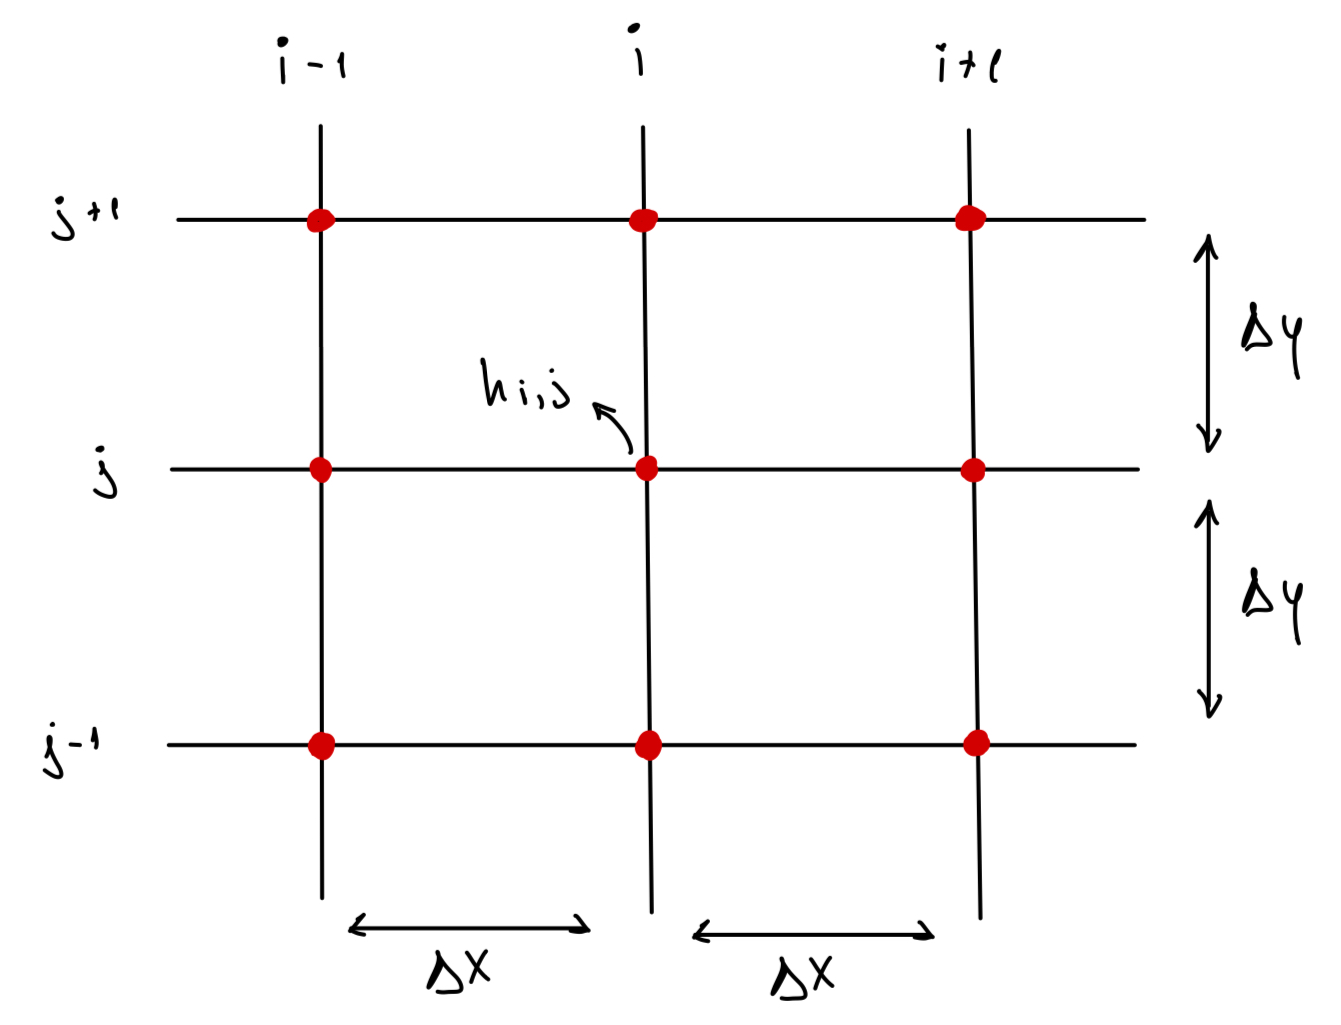
\includegraphics[width=0.5\textwidth]{FOTOS/grilla.jpg}
    \caption{Grilla}
\end{figure}

Donde se puede representar la ecuación de Laplace como:

\begin{equation}
    \frac{d^2h}{dx^2} = \frac{h_{i+1,j} + h_{i-1,j} - 2h_{i,j}}{\Delta x^2}
\end{equation}

\begin{equation}
    \frac{dh}{dx} = \frac{h_{+1,j} + h_{i+1,j}}{2\Delta x}
\end{equation}

Por lo tanto, podemos expresar la ley de Darcy con diferencias centrales, obteniendo:

\begin{equation}
    \frac{k}{\Delta^2}(h_{i+1,j} + h_{i-1,j} + h_{i,j+1} + h_{i,j-1} - 4h_{i,j}) = 0
\end{equation}

Donde se busca:

\begin{equation}
    h_{i,j} = \frac{1}{4}(h_{i+1,j} + h_{i-1,j} + h_{i,j+1} + h_{i,j-1})
\end{equation}

De esta forma, es posible obtener las variaciones en el potencial a partir de los datos conocidos en la grilla (condiciones de borde).

\subsection{Resultados usando Diferencias Finitas}

\subsubsection{Caso 1}

\begin{figure}[H]
    \centering
    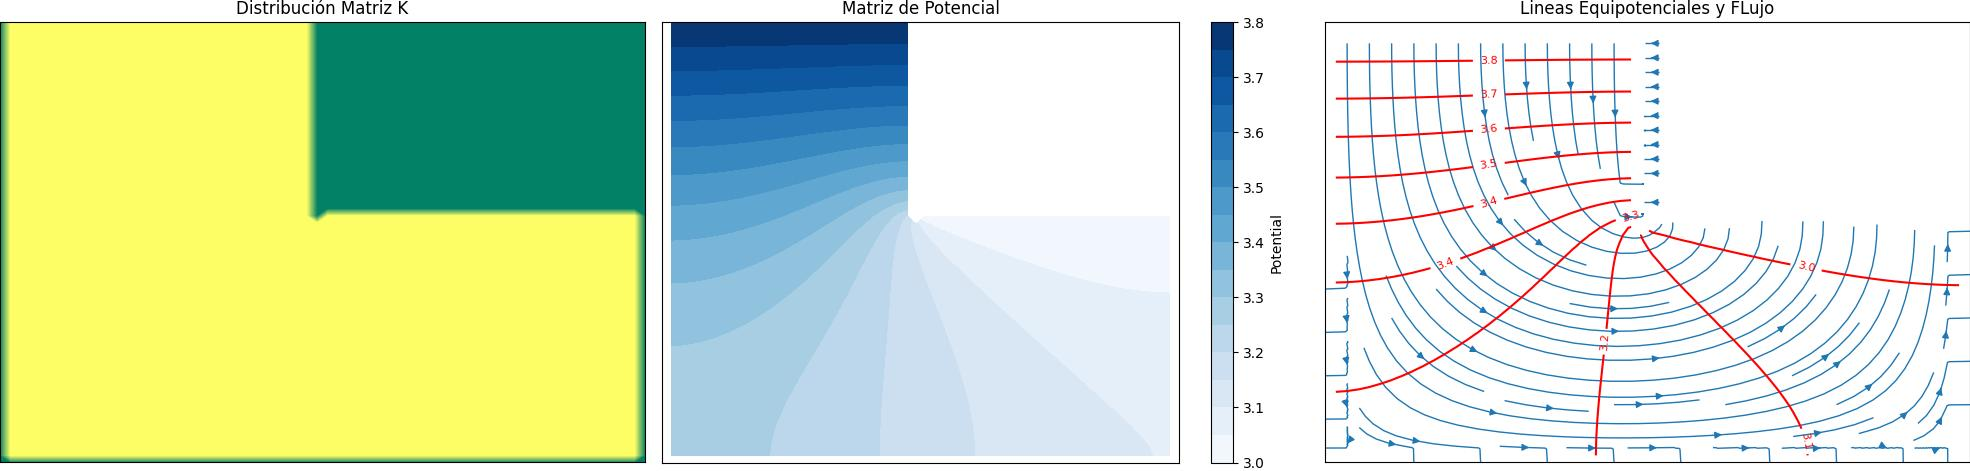
\includegraphics[width=\textwidth]{GRAFICOS/laplace_caso_1.jpg}
    \caption{Caso 1 Laplace}
\end{figure}

\subsubsection{Caso 2}

\begin{figure}[H]
    \centering
    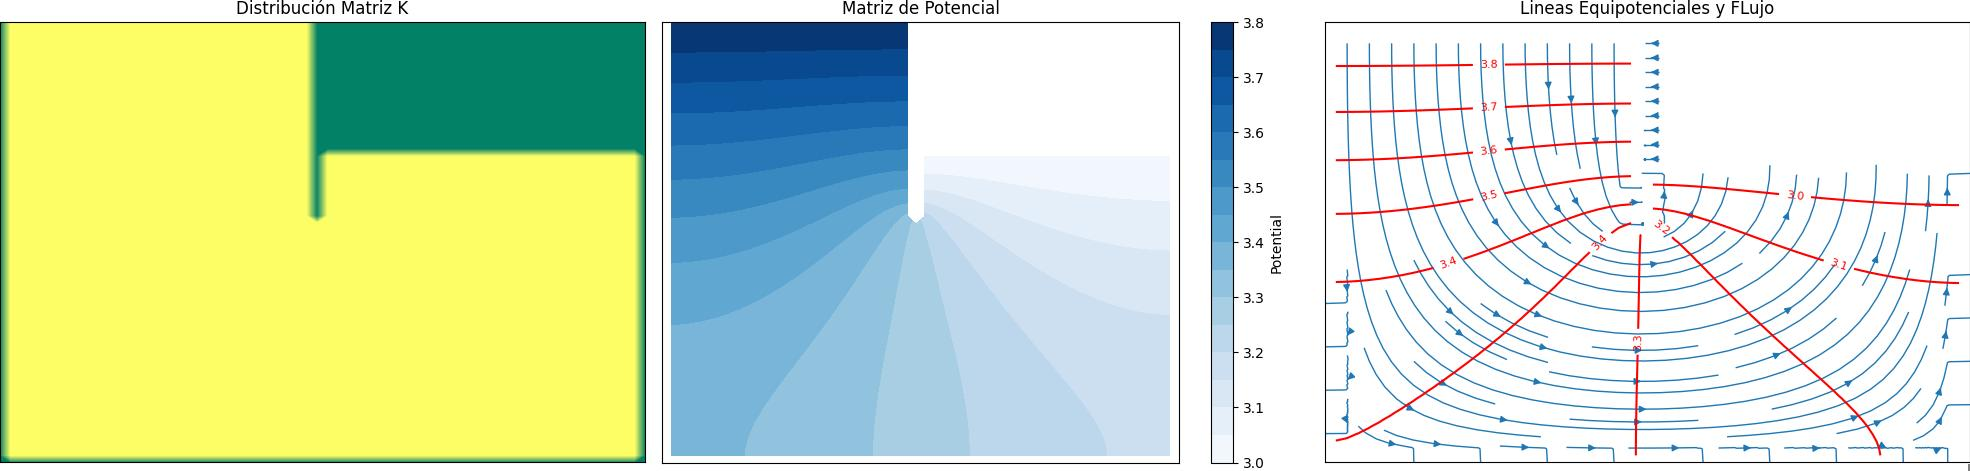
\includegraphics[width=\textwidth]{GRAFICOS/laplace_caso_2.jpg}
    \caption{Caso 2 Laplace}
\end{figure}

\subsubsection{Caso 3}

\begin{figure}[H]
    \centering
    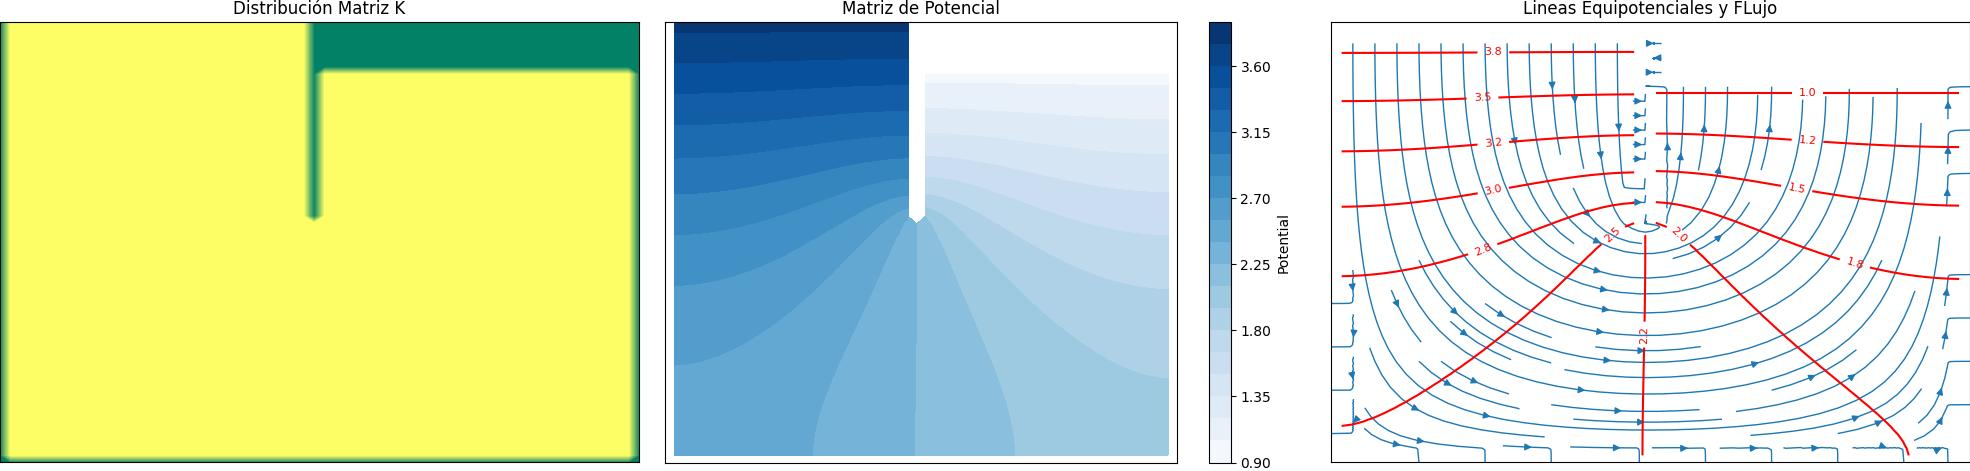
\includegraphics[width=\textwidth]{GRAFICOS/laplace_caso_3.jpg}
    \caption{Caso 3 Laplace}
\end{figure}

\begin{table}[H]
    \begin{center}
        \caption{Gradientes hidráulicos y caudales obtenidos mediante diferencias finitas.}
        \begin{tabularx}{0.75\textwidth}{>{\centering\arraybackslash}X >{\centering\arraybackslash}X >{\centering\arraybackslash}X >{\centering\arraybackslash}X >{\centering\arraybackslash}X }\\
        \hline
        \boldmath{Propiedades} & \boldmath{Caso 1} & \boldmath{Caso 2} & \boldmath{Caso 3} & \boldmath{Unidades} \\
        \hline
        $i_{max}$ & $1.095$ & $0.629$ & $0.380$ & $-$ \\
        $i_{crit}$ & $1.141$ & $1.141$ & $1.141$ & $-$ \\
        $FS$ & $1.041$ & $1.811$ & $2.999$ & $-$\\
        $Q_{inf}$ & $25.410$ & $20.790$ & $13.860$ & $[\frac{m^3}{día}]$\\
        $k$ & $6.9 \times 10^{-5}$ & $6.9 \times 10^{-5}$ & $6.9 \times 10^{-5}$ & $[\frac{m}{s}]$\\
        \hline
        \end{tabularx}
        \label{tab:Diferencias}
    \end{center}
\end{table}

El método de diferencias finitas es una opción de cálculo más precisa que el método manual, ya que incorpora cada parte de la ataguía infinitesimalmente, calculando las presiones de manera más homogénea. Como resultado, se obtuvieron caudales menores y más representativos para cada caso, siendo los casos 1 y 2 caudales relativamente cercanos debido a que la altura de agua en ambos lados de la ataguía es la misma.
